\chapter{Bài toán tối ưu thời gian sống của mạng cảm biến không dây}

\section{Tổng quan về mạng cảm biến không dây}

\begin{figure}[h]
    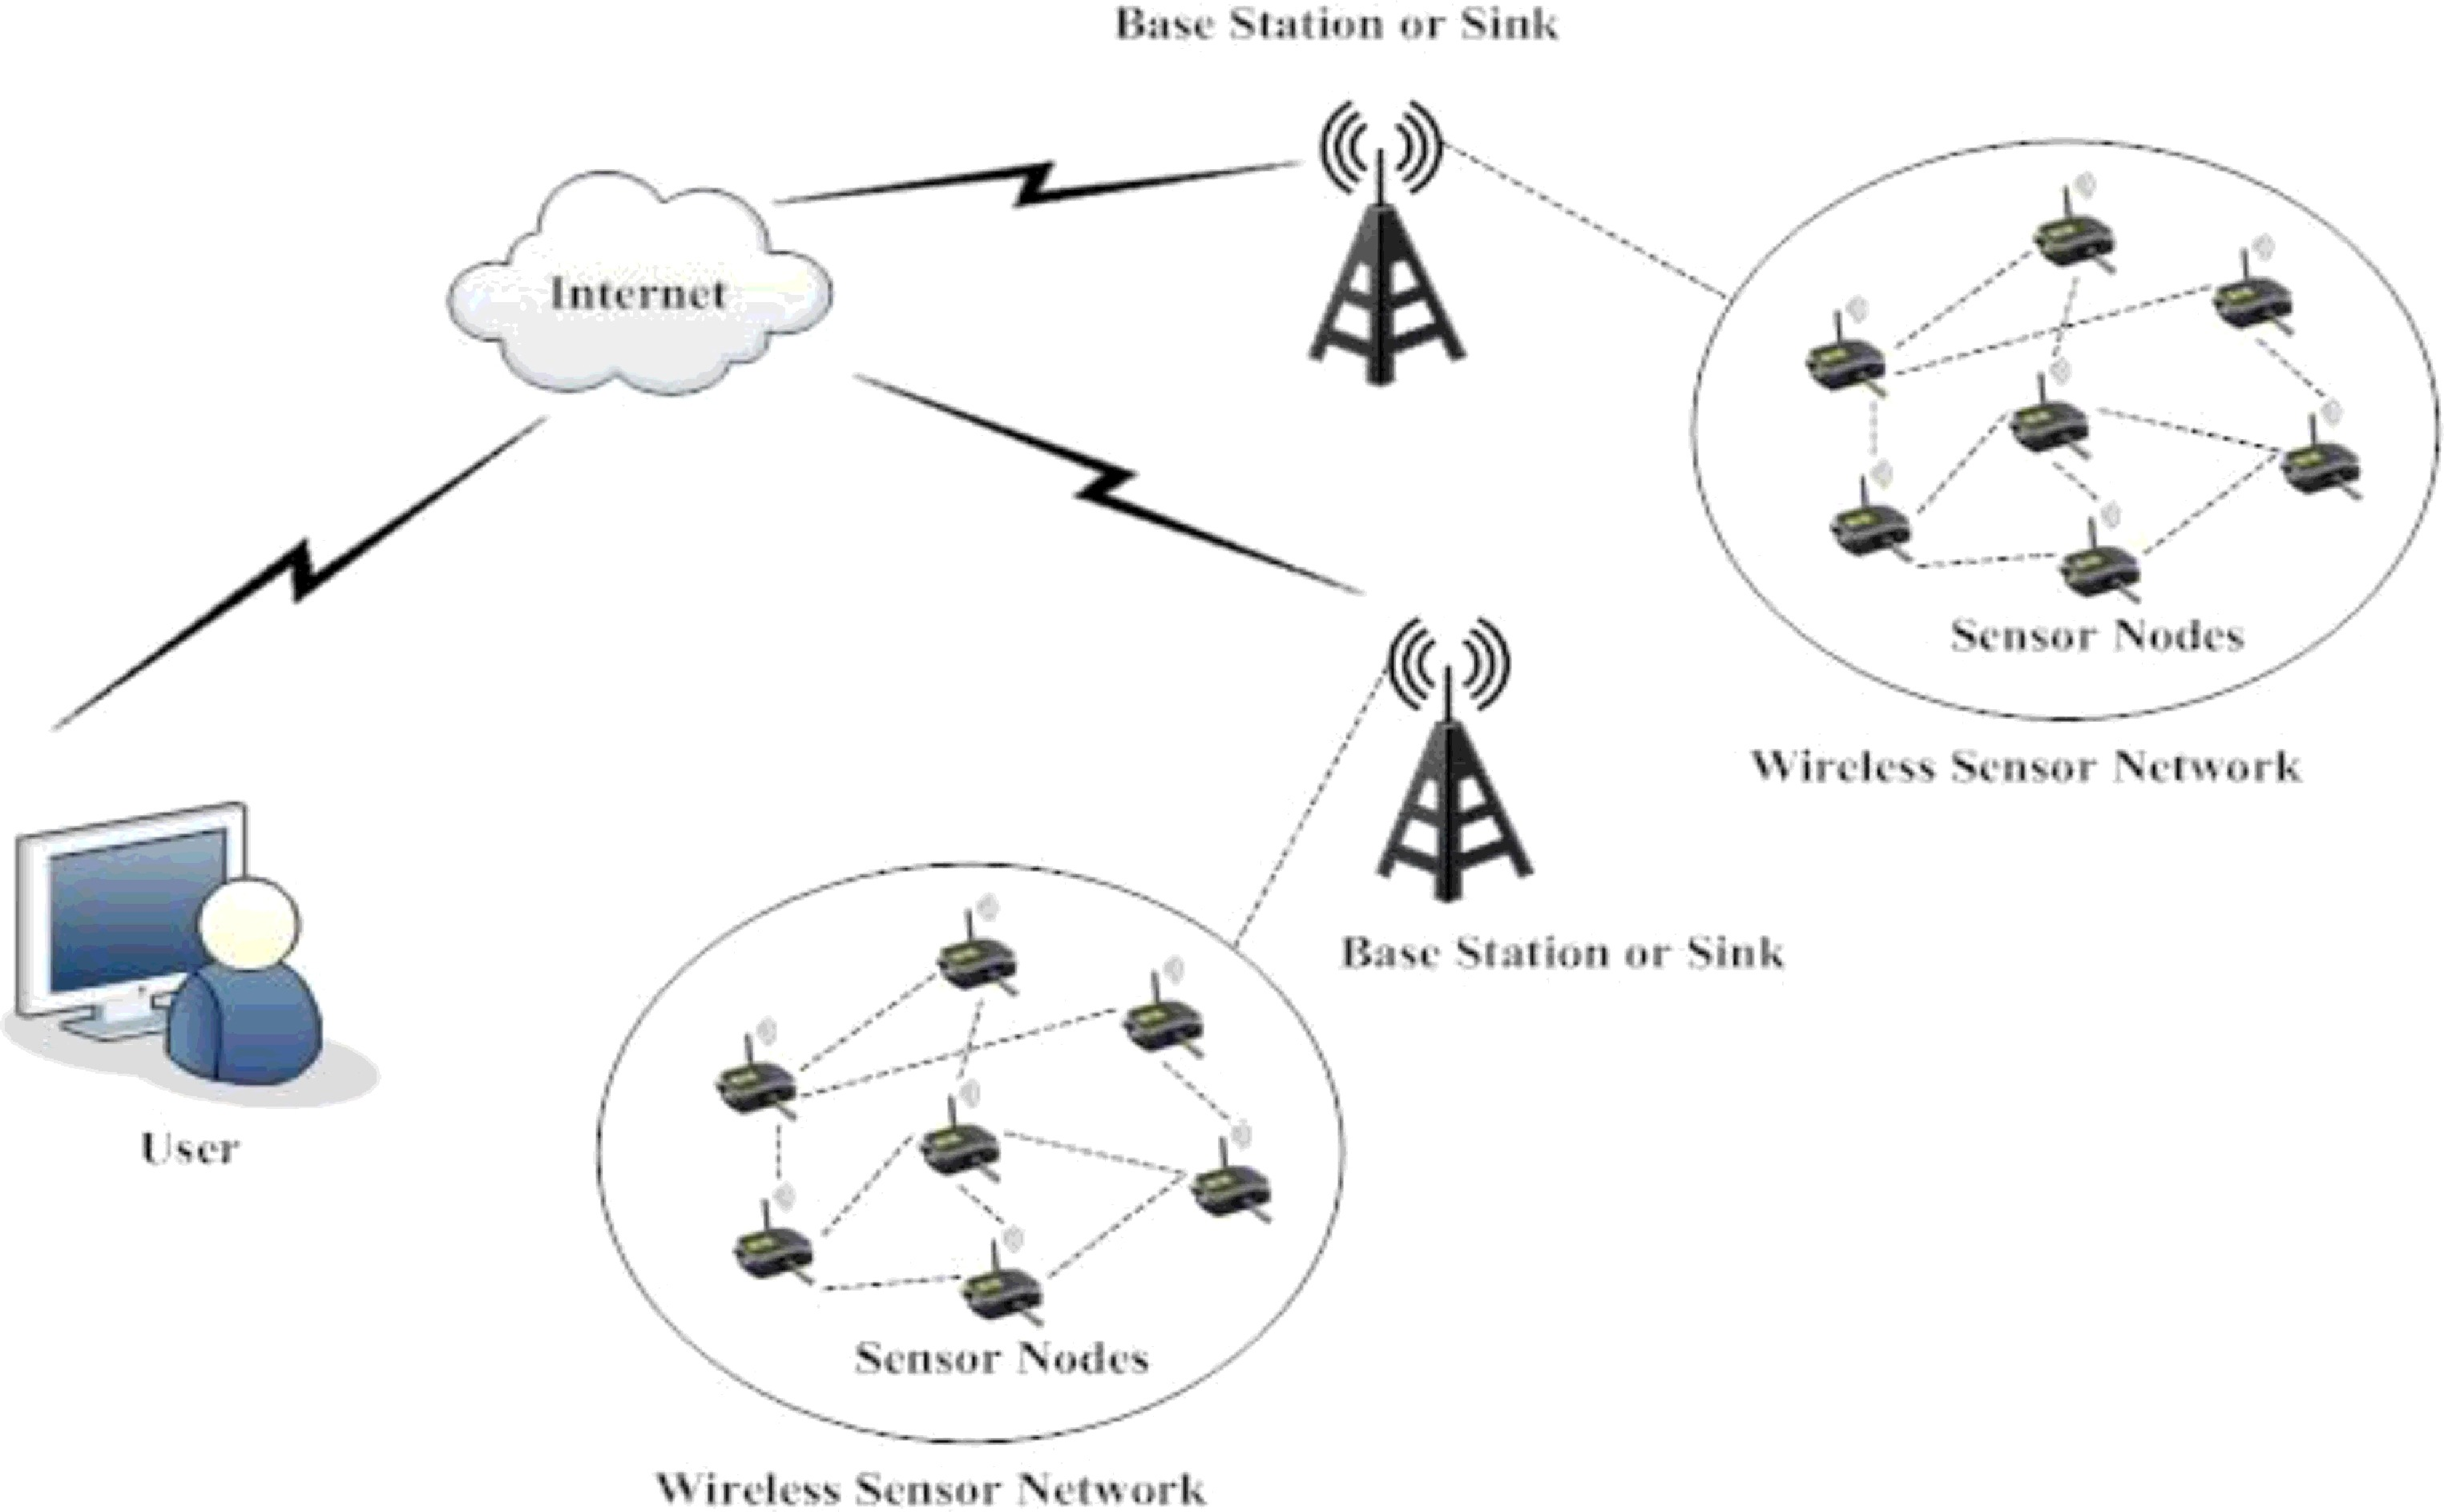
\includegraphics[width=\linewidth]{picture/wsn.jpg}
    \caption{Mạng cảm biến không dây}
    \label{fig:pic1}
\end{figure}
Mạng cảm biến không dây (Wireless Sensor Network - WSN) là mạng liên
kết các nút cảm biến (sensor nodes) với nhau nhờ các liên kết không dây như sóng vô tuyến, hồng ngoại. Các thiết bị cảm biến thường đơn giản, nhỏ gọn, giá thành rẻ và phân bố rộng khắp trong khu vực cảm biến, sử dụng những nguồn năng lượng giới hạn như pin hay ắcquy. Dữ liệu sau khi thu thập được sẽ được gửi đến các trạm cơ sở (Base Stations) trực tiếp hay gián tiếp thông qua một điểm thu phát (Sinks) hoặc các điểm chuyển tiếp (relay nodes) và môi trường mạng công cộng như Internet hay vệ tinh. 
\\Các nút cảm biến không dây có thể được triển khai cho nhiều mục đích chuyên dụng với quy mô khác nhau: giám sát và điều khiển công nghiệp, tự động hóa gia đình và điện dân dụng, quân sự, y tế và giám sát sức khỏe, môi trường và nông nghiệp,... Lợi thế chủ yếu của chúng là có thể triển khai trong rất nhiều môi trường khác nhau, kể cả trong các môi trường nguy hiểm (nhiễm độc, phóng xạ,…) mà mạng có dây truyền thống không thể thực hiện được.
\\ \\\textbf{Cấu trúc của mạng cảm biến không dây}
\\Một mạng cảm biến không dây bao gồm lượng lớn các nút được triển khai dày đặc bên trong khu vực cần thu thập dữ liệu. Vị trí các cảm biến không cần định trước vì vậy nó cho phép triển khai ngẫu nhiên trong các vùng không thể tiếp cận hoặc các khu vực nguy hiểm.
Mỗi nút cảm biến được phát tán trong mạng có khả năng thu thập thông số liệu, định tuyến, số liệu về bộ thu nhận (sink) để chuyển tới người dùng và định tuyến các bản tin mang theo yêu cầu từ nút sink đến các nút cảm biến
\\Mỗi nút cảm biến gồm bốn thành phần cơ bản: bộ cảm biến, bộ xử lý, bộ thu phát sóng không dây và nguồn điện. Tùy theo ứng dụng cụ thể, nút cảm biến còn có thể có các thành phần bổ sung như hệ thống tìm vị trí, bộ sinh năng lượng và thiết bị di động. Bộ cảm biến thường gồm hai đơn vị thành phần là đầu đo cảm biến (sensor) và bộ chuyển đổi tương tự/số (ADC). Bộ xử lý thường kết hợp với một bộ nhớ nhỏ, phân tích thông tin cảm biến và quản lý các thủ tục cộng tác với các nút khác. Bộ thu phát đảm bảo thông tin giữa nút cảm biến và mạng bằng kết nối không dây. Một thành phần quan trọng của nút cảm biến là bộ nguồn, có thể là pin hoặc ắcquy, cung cấp năng lượng cho cảm biến và không thay thế được nên nguồn năng lượng của nút thường là giới hạn. Bộ nguồn có thể được hỗ trợ bởi các thiết bị sinh điện, ví dụ như các tấm pin mặt trời nhỏ.
\\ \\\textbf{Một số đặc điểm của mạng cảm biến không dây}
\\Ưu điểm
\begin{itemize}
    \item Kích thước vật lý nhỏ gọn.
    \item Hoạt động đồng thời với độ tập trung cao.
    \item Dễ dàng triển khai, mở rộng.
    \item Chi phí các thiết bị cảm biến không cao.
    \item Tính đa dạng trong thiết kế và sử dụng.
    \item Hoạt động tin cậy.
\end{itemize}
Nhược điểm
\begin{itemize}
    \item Khả năng liên kết vật lý và phân cấp điều khiển hạn chế.
    \item Thiết bị cảm biến có khả năng tính toán, lưu trữ và nguồn năng lượng hạn chế.
    \item Dư thừa dữ liệu.
    \item Truyền thông không dây dẫn tới một số vấn đề như độ ổn định, mất mát thông tin, bảo mật.
\end{itemize}
\section{Bài toán tối ưu thời gian sống của mạng cảm biến không dây }
Với sự phát triển mạnh mẽ của mình, mạng cảm biến không dây được ứng dụng vào rất nhiều lĩnh vực khác nhau như nông nghiệp, quân sự, y tế… Và để sử dụng một cách hiệu quả, rất nhiều vấn đề trong mạng cảm biến không dây được quan tâm nghiên cứu như hiệu suất, độ bao phủ, cấu trúc mạng, phương thức định tuyến… trong đó có một trong các yếu tố quan trọng bậc nhất đó là vấn đề năng lượng hay nói cách khác là thời gian sống (tuổi thọ) của mạng cảm biến, do một mạng cảm biến chỉ thực thi đầy đủ chức năng của mình khi nó còn “sống”. Cho đến nay có nhiều cách định nghĩa về tuổi thọ của mạng cảm biến không dây khác nhau do nhiều tác giả đưa ra. Ta sẽ đề cập một số cách định nghĩa phổ biến sau.
\subsection{Tuổi thọ của mạng dựa vào số nút còn hoạt động}
Cách định nghĩa phổ biến trong các tài liệu đó là $n-of-n$, trong đó tuổi thọ của mạng được định nghĩa bằng tuổi thọ của nút cảm biến có thời gian sống ít nhất.
\[T_n^n = \min_{v \in V} T_v\]
Trong đó $T_n$ là thời gian sống của nút $v$.
\\$T_n^n$ là cách định nghĩa đơn giản và thuận tiện cho tính toán, các thuật toán dùng trong mạng không cần quan tâm đến bất kì sự thay đổi nào của kiểu hình mạng. Tuy nhiên trong phần lớn trường hợp, cách định nghĩa này có ý nghĩa lớn trong các bài toán lí thuyết hơn là các ứng dụng thực tế của mạng cảm biến. Ví dụ, xét một nút cảm biến có nhiều nút hàng xóm với công năng cảm biến tương đương, nhiều mạng cảm biến hoàn toàn có thể chấp nhận được việc nút này dừng hoạt động và sử dụng các nút hàng xóm, nhưng  không xét đến các trường hợp như vậy và cho rằng mạng đã “chết”. Do đó, ta nên sử dụng cách định nghĩa này khi các nút trong mạng có độ quan trọng xấp xỉ nhau.
\\Ngoài ra còn có một số biến thể khác của $T_n^n$. Tuổi thọ của mạng được định nghĩa là thời gian nhỏ nhất của một nút từ khi bắt đầu hoạt động cho đến khi năng lượng của nút xuống thấp hơn một mức $\beta$ cho trước, hoặc cũng có thể được định nghĩa mạng còn sống khi ít nhất $k$ nút trong mạng còn hoạt động ($k-of-n - T_n^k$).
\subsection{Tuổi thọ của mạng dựa vào độ bao phủ của các nút cảm biến}
Trong khi đánh giá tuổi thọ của mạng cảm biến dựa vào số nút cảm biến còn hoạt động là một cách định nghĩa khá tổng quát thì việc xét đến các đặc điểm của mạng cảm biến, cụ thể như đánh giá tuổi thọ của mạng dựa vào độ bao phủ của các nút cảm biến với môi trường đang khảo sát có vẻ như là một cách tự nhiên hơn để định nghĩa tuổi thọ của mạng.
\\Các mô hình bao phủ trong mạng cảm biến có thể chia thành ba loại chính:
\begin{itemize}
    \item Bao phủ diện tích: mỗi điểm trong không gian khảo sát đều phải nằm trong vùng cảm biến.
    \item Bao phủ đối tượng: một số điểm định trước trong không gian phải nằm trong vùng cảm biến.
    \item Bao phủ barrier: mạng cảm biến cần có chức năng phát hiện đối tượng di chuyển vào hoặc băng qua khu vực được giám sát.
\end{itemize}
Có hai cách để mô tả độ bao phủ của một mạng cảm biến:
\begin{itemize}
    \item Một số phần trăm $\alpha$ của không gian được bao phủ bởi ít nhất một cảm biến, thường được gọi là $\alpha-coverage$.
    \item Mỗi điểm trong không gian cần được bao phủ bởi ít nhất k sensor, thường được gọi là $k-coverage$.
\end{itemize}
Nhiều nghiên cứu định nghĩa tuổi thọ của mạng dựa trên các biến thể của cách định nghĩa trên, trong đó phổ biến nhất là 1-coverage, tức là tuổi thọ của mạng được tính từ lúc bắt đầu triển khai cho đến khi tất cả các điểm cần thiết nằm trong vùng cảm biến của ít nhất một nút cảm biến.
\\Độ bao phủ thường là một yếu tố cực kì quan trọng để đánh giá hiệu quả của mạng cảm biến, tuy nhiên đánh giá tuổi thọ của mạng chỉ dựa trên độ bao phủ thì không hợp lí, do không thể đảm bảo dữ liệu thu thập được chắc chắn truyền về nút sink.
\subsection{Tuổi thọ của mạng dựa trên kết nối }
\cite{Baydere2005} và \cite{Yu2001} định nghĩa tuổi thọ của mạng dựa trên tổng số lượng gói tin có thể truyền tới nút sink. Mặc dù số lượng này có thể đóng vai trò là chỉ số cho sự bền bì của mạng, nhưng nó phụ thuộc rất nhiều vào các thuật toán cụ thể được áp dụng trong mạng. Giả sử ta áp dụng thuật toán tập hợp thông tin trong mạng, như vậy số gói tin truyền về nút sink sẽ giảm trong khi lượng thông tin nhận được vẫn là tương đương. Do đó khả năng áp dụng định nghĩa này trong việc so sánh tuổi thọ của các thiết lập mạng khác nhau sẽ bị hạn chế.
\\Một nhược điểm khác của cách định nghĩa này là số các gói tin được truyền về không phản ánh được mạng cảm biến hoạt động bình thường trong bao lâu (tính theo đơn vị thời gian).
\\Trong \cite{Giridhar} định nghĩa tuổi thọ của mạng dựa theo số lần thu thập dữ liệu từ môi trường thành công, trong đó với mỗi lần thu thập dữ liệu thì không có nút nào hết năng lượng. Cách định nghĩa này có thể quy dẫn về $T_n^n$ đã nêu ở trên, chỉ khác đó là tuổi thọ không được tính theo đơn vị thời gian mà là số lần thu thập dữ liệu.
\subsection{Tuổi thọ của mạng dựa trên độ bao phủ của các nút cảm biến và kết nối}
Do một số hạn chế của việc đánh giá tuổi thọ mạng dựa trên độ bao phủ hoặc dựa vào kết nối, một số tác giả đã kết hợp cả hai tiêu chí này lại để đánh giá tuổi thọ của mạng cảm biến. Trong \cite{Wang2003}, tuổi thọ của mạng định nghĩa bằng thời gian từ khi mạng bắt đầu hoạt động cho tới khi độ bao phủ hoặc kết nối hạ xuống thấp hơn ngưỡng cho trước, trong đó độ bao phủ sử dụng $\alpha-coverage$ và kết nối sử dụng tỉ lệ số gói nhận được tại sink so với tổng số gói được gửi từ các nút cảm biến.
\subsection{Tuổi thọ của mạng dựa trên chất lượng ứng dụng}
Một số nghiên cứu định nghĩa tuổi thọ của mạng cảm biến dựa trên chất lượng ứng dụng, cách định nghĩa này gần với thực tế nhất do mọi thiết kế, kiến trúc của mạng cảm biến đều phụ thuộc vào ứng dụng cụ thể mà mạng thực hiện. Ví dụ trong \cite{Giridhar} đã nêu ``tuổi thọ của mạng cảm biến là khoảng thời gian mà nó thực thi các yêu cầu của ứng dụng một cách bình thường''. Tuy nhiên, cách định nghĩa này khó có thể áp dụng trong các nghiên cứu lí thuyết do nó quá trừu tượng và gần như không thể mô hình hóa được.
\section{Các nghiên cứu liên quan }
Năm 2017, Bo Yuan và cộng sự \cite{xin_yao_paper} đưa ra mô hình bài toán với mạng cảm biến không dây ngầm. Nội dung như sau: xét một mạng cảm biến không dây ngầm, trong đó có một số cảm biến (sensors) được chôn dưới lòng đất và trên mặt đất có các vị trí khả thi để đặt nút chuyển tiếp (relays), ngoài ra có các trạm cơ sở (base stations), thông tin thu nhận từ các cảm biến được chuyển tiếp qua các nút relays để gửi đến base stations, cho biết trước số lượng relays được triển khai, mục tiêu đặt ra là tìm vị trí thích hợp để triển khai các nút này sao cho tuổi thọ của mạng được tối ưu hóa.
\\Trong mô hình này, tác giả đưa ra giả thiết trong địa hình đã cho, bất kì cặp sensor - relay nào cũng đều có thể kết nối được với nhau, số relays được triển khai là cố định cho trước, do đó để tối ưu thời gian sống của mạng, tác giả sử dụng điều kiện cân bằng tải, tức là mỗi relay sẽ kết nối đến số sensors bằng nhau.
\\Bài toán đã được chứng minh là NP-Khó. Tác giả đưa ra cách giải quyết theo hai pha:
\begin{itemize}
    \item Pha một: giải quyết bài toán, tạo các kết nối mà không xét đến điều kiện cân bằng tải.
    \item Pha hai: sắp xếp lại các kết nối để duy trì điều kiện cân bằng tải.
\end{itemize}
Với pha một, tác giả đưa ra hai đề xuất heuristics:
\begin{itemize}
    \item Lần lượt triển chọn các vị trí để triển khai relay sao cho năng lượng tiêu hao lớn nhất trong mạng là nhỏ nhất, cho đến khi đủ số relay cần triển khai.
    \item Kết nối một sensor với relay gần nó nhất, sau đó nếu số relay kết nối nhiều hơn số relay được triển khai, loại bỏ dần bằng cách tính toán sao cho năng lượng tiêu hao lớn nhất trong mạng là nhỏ nhất.
\end{itemize}
Với pha hai, tác giả đưa ra ba đề xuất heuristics:
\begin{itemize}
    \item Với các relay đã quá tải, chuyển dần các sensor của relay này cho các relay thiếu tải.
    \item Với các relay thiếu tải, lấy lần lượt các sensor ở relay đã quá tải.
    \item Tính toán một điểm là trung tâm của mạng, sau đó tính khoảng cách từ các relay đến trung tâm điểm này, xét từ relay xa nhất tới relay gần nhất, nếu relay đó đã quá tải thì sử dụng đề xuất một cho relay đó, nếu relay thiếu tải thì sử dụng đề xuất hai.
\end{itemize}
Dễ nhận thấy một điểm chưa khả thi trong mô hình này, đó là mỗi cặp relay-sensor trong mạng đều có thể kết nối được với nhau, nếu một cặp relay-sensor nằm ở hai góc khác nhau ở địa hình thì việc có thể kết nối được với nhau là khó xảy ra trong trường hợp địa hình lớn. Trên cơ sở đó đồ án đề xuất một mô hình mới như sau.
\section{Mô hình bài toán tối ưu tuổi thọ mạng cảm biến không dây ngầm}
Nội dung bài toán: cho một mạng cảm biến gồm $n$ cảm biến được triển khai ngầm trong lòng đất, trên mặt đất có một tập các vị trí khả thi để đặt nút chuyển tiếp. Nhiệm vụ của các nút chuyển tiếp là nhận dữ liệu từ các nút cảm biến sau đó gửi đến trạm cơ sở ở trung tâm của mạng. Bài toán đặt ra là cần chọn một tập các vị trí trong các vị trí khả thi để triển khai nút chuyển tiếp nhằm kéo dài thời gian sống của mạng và số các nút chuyển tiếp cần dùng là ít nhất có thể.
\\Tuổi thọ của mạng sử dụng định nghĩa $T_n^n$ đã nêu ở trên. Với cách định nghĩa này, mạng dừng hoạt động khi có một nút hết năng lượng. Có nhiều cách tiếp cận để giải quyết bài toán với định nghĩa tuổi thọ $T_n^n$. Trong mô hình này ta sử dụng cách tiếp cận tối thiểu hóa năng lượng tiêu hao cực đại của một nút trong mạng.
\\Với mục tiêu tối ưu hai mục tiêu cùng lúc là thời gian sống tối đa và số nút chuyển tiếp cần dùng tối thiểu, nếu giá trị của hàm mục tiêu là một bộ gồm hai giá trị số thực, ta khó có thể so sánh một tập các lời giải gần tương đương nhau để đánh giá lời giải nào tốt hơn, do đó ta sẽ đưa hàm mục tiêu về dạng số thực nhằm thuận tiện cho việc đánh giá.
\\ \textbf{Đầu vào }
\begin{itemize}
    \item Không gian 3 chiều cần khảo sát với chiều dài và chiều rộng lần lượt là $W$ và $H$, chiều cao (sâu) vô hạn.
    \item $S = \{s_1, s_2,…, s_n\}$: tập các nút cảm biến được triển khai, mỗi nút cảm biến $s_i$ có các thuộc tính:
    \begin{itemize}
        \item[] $(xs_i, ys_i)$: tọa độ trên mặt $Oxy$
        \item[] $hs_i$: độ sâu so với mặt đất của cảm biến
        \item[] $r$: bán kính truyền thông 
        \item[] $l$: số bit mà nút cảm biến gửi tới trạm cơ sở
    \end{itemize}
    \item $F = \{f_1, f_2,…, f_m\}$: tập các vị trí khả thi để triển khai các nút chuyển tiếp, $f_i$ gồm các thuộc tính:
    \begin{itemize}
        \item[] $(xr_i, yr_i)$: tọa độ trên mặt $Oxy$
        \item[] $hr_i$: độ cao so với mặt đất của cảm biến
        \item[] $R$: bán kính truyền thông 
    \end{itemize}
    \item $D = \{d_{11}, d_{12},…, d_{nm}\}$: ma trận khoảng cách 
    \begin{itemize}
        \item[] $d_{ij}$: khoảng cách từ sensor $s_i$ đến relay $f_j$
    \end{itemize}
    \item $C = \{c_{11}, c_{12},…, c_{nm}\}$: ma trận kết nối
    \begin{equation} 
        c_{ij} = \begin{cases}
            1 & \textrm{nếu $d_{ij} \leq r_i + R_j$}\\
            0 & \textrm{nếu ngược lại}
        \end{cases}
        \label{eqn:simple_one} 
    \end{equation}     
    \begin{itemize}
        \item[] Ý nghĩa: sensor $s_i$ có thể kết nối với relay $f_j$ nếu khoảng cách giữa hai nút không vượt quá tổng bán kính truyền thông của chúng
    \end{itemize}
    \item Năng lượng tiêu hao khi truyền $l$ bits dữ liệu từ sensor $s_i$ đến relay triển khai tại $f_j$
    \begin{equation}
        Et_{ij} = l * (E_{TX} + e_{fs} * d_{ij}^2)
        \label{sensor_consumption}
    \end{equation}
    \item Năng lượng tiêu hao của relay triển khai tại $f_j$ nhận dữ liệu từ $x_j$ sensors, tổng hợp và gửi tới trạm cơ sở
    \begin{equation}
        Er_j = l * (x_j * E_{RX} + x_j * E_{DA} + e_{mp} * d_{jtoBS}^4)
        \label{relay_consumption}
    \end{equation}
    \item $E_{max}$: năng lượng tiêu thụ tối đa mà một nút trong mạng có thể đạt đến
\end{itemize}
\textbf{Đầu ra }
\begin{itemize}
    \item $z = (z_1, z_2,…, z_m)$: vector quyết định
    \begin{equation}
        z_j = \begin{cases}
            1 & \textrm{nếu có relay triển khai tại $f_j$}\\
            0 & \textrm{nếu ngược lại}
        \end{cases}
    \end{equation}
    \item $A = \{a_{11}, a_{12},…, a_{nm}\}$: ma trận quyết định
    \begin{equation}
        a_{ij} = \begin{cases}
            1 & \textrm{nếu $s_i$ kết nối tới $f_j$}\\
            0 & \textrm{nếu ngược lại}
        \end{cases}
    \end{equation}
\end{itemize}
\textbf{Ràng buộc }

\begin{equation}
    \sum_{j = 0}^m a_{ij} = 1 ~\forall i = 0, 1, \ldots, n: \textrm{mỗi sensor chỉ kết nối tới 1 relay}
\end{equation}
\begin{equation}
    z_j = a_{1j} \wedge a_{2j} \wedge \ldots \wedge a_{nj} ~\forall j = 1, 2, \ldots, m
\end{equation}

\textbf{Hàm mục tiêu }

\begin{equation}
    \frac{\alpha}{m} * \sum_{j = 1}^m z_j + \frac{1 - \alpha}{E_{max}} * E_x \rightarrow min
    \label{obj_func}
\end{equation}

Trong đó:
\begin{itemize}
    \item $E_x$ là năng lượng tiêu  hao lớn nhất của một nút trong lời giải. 
    \item $0 \leq \alpha \leq 1$: trọng số đánh giá độ quan trọng của số nút chuyển tiếp được sử dụng.
\end{itemize}

Ý tưởng giải quyết bài toán: khi sử dụng hàm mục tiêu đã nêu trong công thức \ref{obj_func}, giá trị của hàm mục tiêu phụ thuộc vào năng lượng tiêu hao và số relays sử dụng, do đó trong bài toán này ta cần giải quyết hai vấn đề: vị trí nào được chọn để triển khai relay và kết nối giữa các relay và sensor. Đồ án đưa ra phương pháp giải quyết theo hai pha
\begin{itemize}
    \item Pha một: xác định các vị trí được chọn để triển khai relays.  
    \item Pha hai: xác định kết nối giữa sensors và relays. 
\end{itemize}